% Provenance (never printed): cycle 3 / 6e "La planete Terre" (rocks and
% minerals; the three rock families; recognising common rocks); see
% sources/book1/PROVENANCE.md. Book 1, grade 6, chapter 3.
% Vocabulary guard: "magma" not before g7.2 (here "molten rock");
% "sediment" not before g7.4 (here "grains of sand and mud").
\chapter{Rocks and Minerals}\label{ch:g6:rocks-and-minerals}

Sam leans over the kitchen worktop with a hand lens. The polished stone,
which looks grey from far away, turns into a crowd of specks: pink ones,
white ones, glassy grey ones and tiny black ones that shine when the light
catches them. Each speck has flat, shiny faces, and the specks fit together
like the pieces of a jigsaw. What are they?

\begin{omfigure}
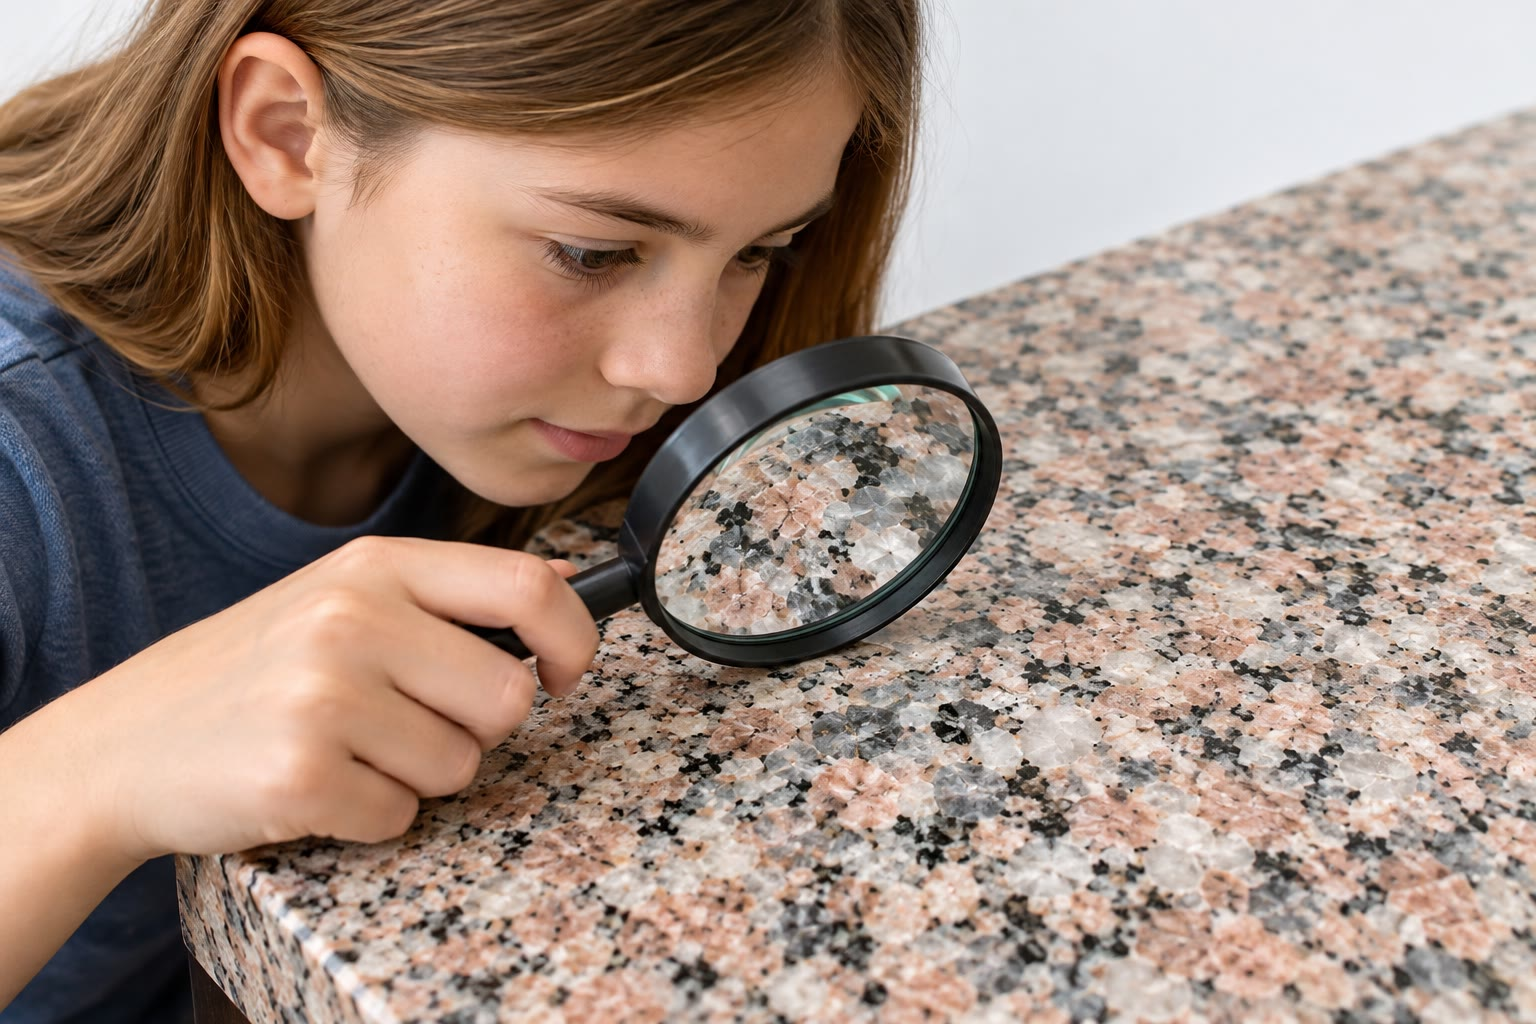
\includegraphics[width=0.6\linewidth]{images/book1/ai/g6-hand-lens-worktop.jpg}

{\small Looking at a speckled stone worktop through a hand lens. (AI
illustration.)}
\end{omfigure}

\begin{recall}
\omterm{def:g3:stones-pebbles-sand:rock}{Rocks} are the hard material of the Earth's crust: they can be broken into
stones, rolled by \omterm{def:g1:landscapes-around-us:water}{rivers} into \omterm{def:g3:stones-pebbles-sand:pebble}{pebbles}, and ground into \omterm{def:g3:stones-pebbles-sand:sand}{sand}
(\cref{ch:g3:stones-pebbles-sand}). Water, ice and wind wear \omterm{def:g3:stones-pebbles-sand:rock}{rocks} away
(\omterm{def:g5:water-shapes-the-land:weathering}{weathering}), carry the pieces off (\omterm{def:g5:water-shapes-the-land:erosion}{erosion}) and drop them further down
(\omterm{def:g5:water-shapes-the-land:deposition}{deposition}) (\cref{ch:g5:water-shapes-the-land}). At a \omterm{def:g4:volcanoes-earthquakes-first-look:volcano}{volcano}, molten
\omterm{def:g3:stones-pebbles-sand:rock}{rock} comes out as \omterm{def:g4:volcanoes-earthquakes-first-look:eruption}{lava} (\cref{ch:g4:volcanoes-earthquakes-first-look}).
\end{recall}

\section{A rock is made of minerals}

The specks of the worktop are \omterm{def:g6:rocks-and-minerals:mineral}{minerals}, and the stone is a granite.

\begin{definition}[Mineral]\label{def:g6:rocks-and-minerals:mineral}
A \emph{mineral}\index{mineral} is a natural solid substance, not made by
living things, always with the same make-up and with its atoms arranged in
a regular way. A \emph{\omterm{def:g3:stones-pebbles-sand:rock}{rock}} is made of one mineral or, more often, of
several minerals stuck together.
% ledger: usgs:mineral-rock
\end{definition}

Granite is made mostly of three \omterm{def:g6:rocks-and-minerals:mineral}{minerals}: \emph{feldspar} (pink or white),
\emph{quartz} (grey and glassy) and \emph{mica} (black or silvery, in thin
shiny flakes). Other \omterm{def:g3:stones-pebbles-sand:rock}{rocks} are made of a single \omterm{def:g6:rocks-and-minerals:mineral}{mineral}: limestone, for
example, is made almost only of calcite.
% ledger: nps:granite-minerals, usgs:mineral-rock

\begin{omfigure}
\begin{minipage}[c]{0.5\linewidth}\centering
\begin{tikzpicture}
  \begin{axis}[axis equal image, hide axis, width=\linewidth,
      xmin=0, xmax=6, ymin=0, ymax=4]
    \addplot[fill=orange!35!pink, draw=black!55, line width=0.4pt]
      table {figdata/out/grade-6-granite_mosaic-feldspar.dat};
    \addplot[fill=black!12, draw=black!55, line width=0.4pt]
      table {figdata/out/grade-6-granite_mosaic-quartz.dat};
    \addplot[fill=black!85, draw=black!55, line width=0.4pt]
      table {figdata/out/grade-6-granite_mosaic-mica.dat};
  \end{axis}
\end{tikzpicture}

{\small \tikz\fill[orange!35!pink, draw=black!55] (0,0) rectangle (0.25,0.18); feldspar\quad
\tikz\fill[black!12, draw=black!55] (0,0) rectangle (0.25,0.18); quartz\quad
\tikz\fill[black!85] (0,0) rectangle (0.25,0.18); mica}
\end{minipage}\hfill
\begin{minipage}[c]{0.46\linewidth}\centering
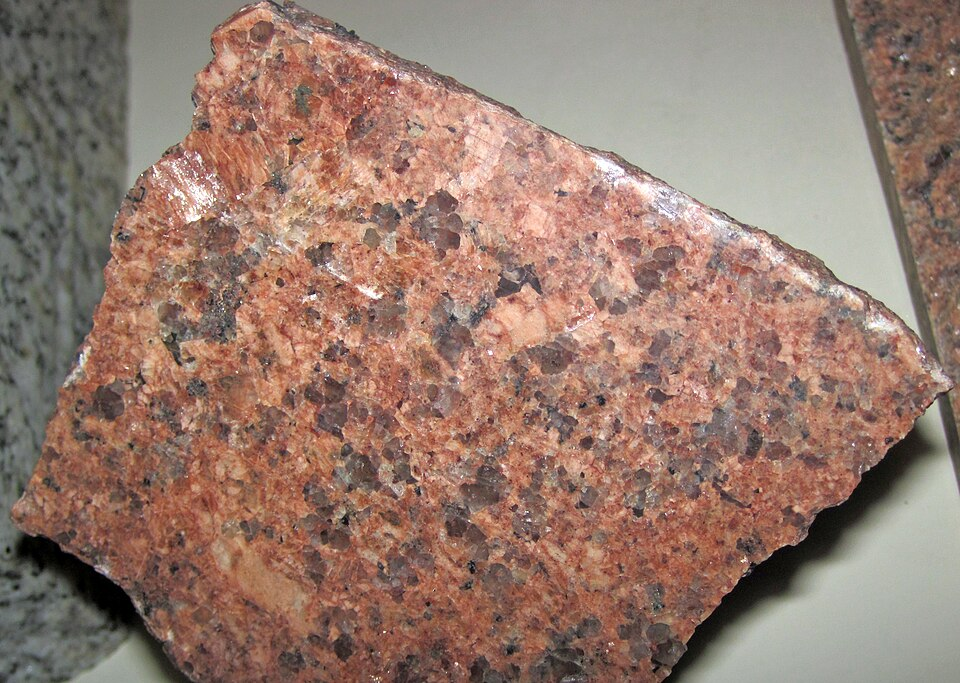
\includegraphics[width=\linewidth]{images/book1/g6-granite.jpg}
\end{minipage}

\smallskip
{\small Left: granite drawn as a mosaic of grains, each grain one \omterm{def:g6:rocks-and-minerals:mineral}{mineral}
(an enlargement, not to scale). Right: a real pink granite, about the size
of a hand. (Photo: James St.~John, CC BY 2.0, via Wikimedia Commons.)}
% ledger: nps:granite-minerals, commons:jsj-rocks (figdata/grade-6/granite_mosaic.py)
\end{omfigure}

\section{Crystals}

Under the lens, many \omterm{def:g6:rocks-and-minerals:mineral}{mineral} grains show flat, shiny faces and straight
edges. Where a \omterm{def:g6:rocks-and-minerals:mineral}{mineral} has had room to grow freely, in a hollow of the
\omterm{def:g3:stones-pebbles-sand:rock}{rock}, it forms a crystal: a solid with a regular shape bounded by flat
faces. Its shape comes from the regular arrangement of its atoms, studied
in the chemistry books. A quartz crystal, for example, is a column with six
sides ending in a point; a mica crystal splits into sheets thinner than
paper.

\begin{omfigure}
\begin{minipage}[c]{0.2\linewidth}\centering
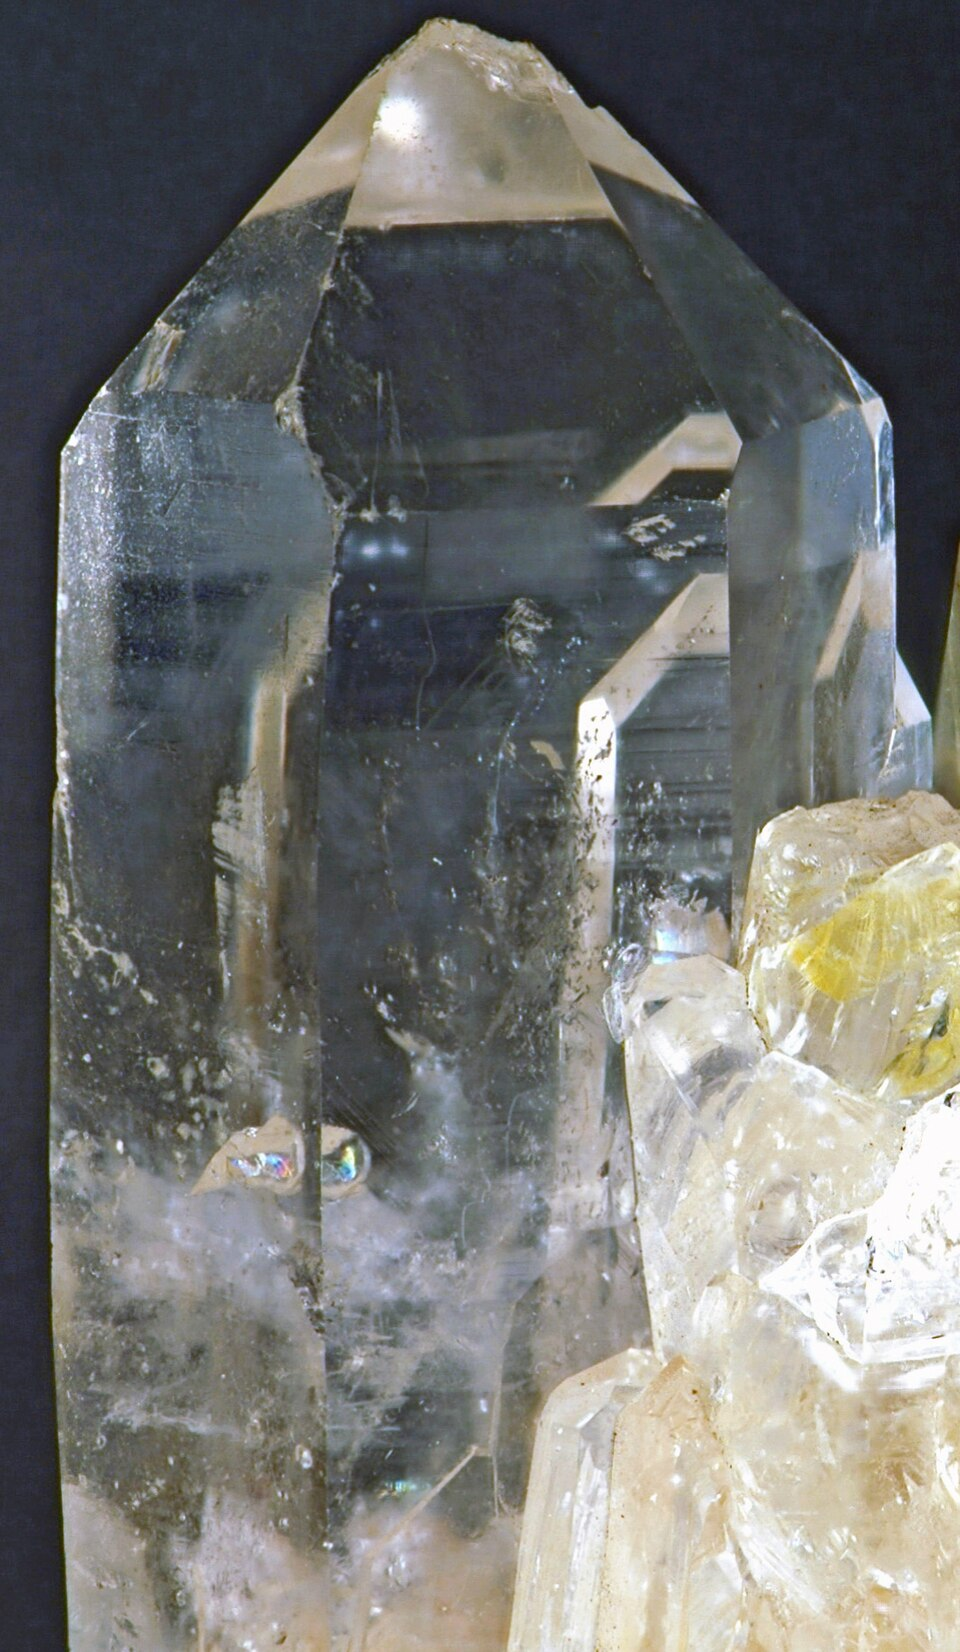
\includegraphics[height=4.2cm]{images/book1/g6-quartz.jpg}
\end{minipage}\hfill
\begin{minipage}[c]{0.44\linewidth}\centering
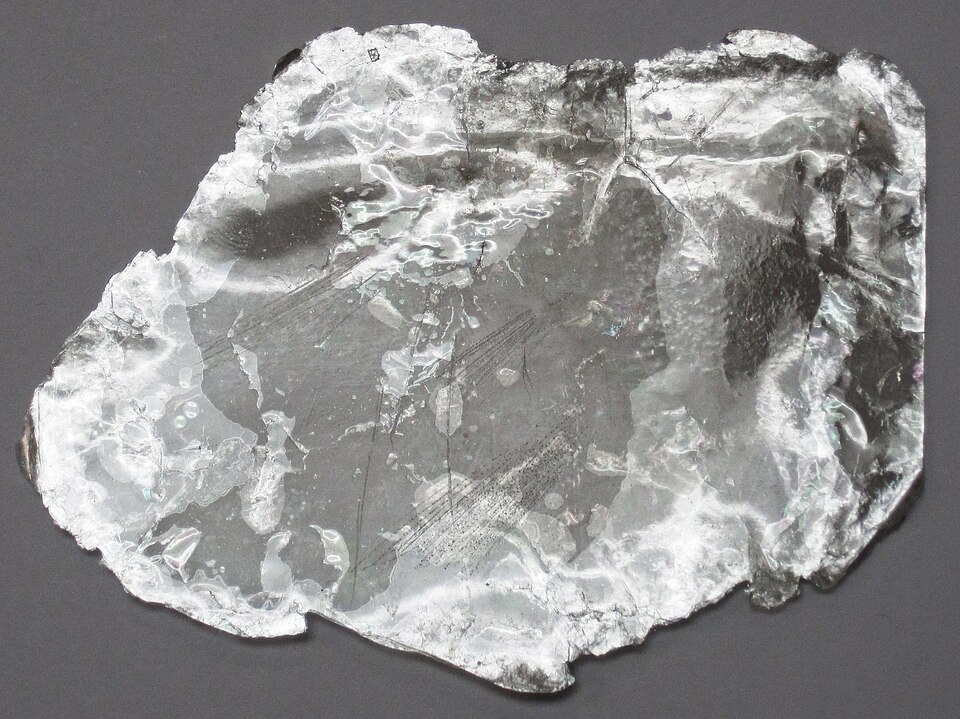
\includegraphics[height=4.2cm]{images/book1/g6-mica.jpg}
\end{minipage}\hfill
\begin{minipage}[c]{0.28\linewidth}
{\small Left: a quartz crystal, with its flat faces. Right: a sheet of
mica, a \omterm{def:g6:rocks-and-minerals:mineral}{mineral} that splits into very thin flakes. (Photos: James
St.~John, CC BY 2.0, via Wikimedia Commons.)}
% ledger: commons:jsj-rocks
\end{minipage}
\end{omfigure}

In granite, the grains grew pressed against each other, so they are not
nicely shaped: they fit together like a jigsaw. Their size tells a story.
Granite forms deep underground, where molten \omterm{def:g3:stones-pebbles-sand:rock}{rock} cools very slowly: its
grains have time to grow large enough to be seen with the eye. Molten \omterm{def:g3:stones-pebbles-sand:rock}{rock}
that cools quickly at the surface, as \omterm{def:g4:volcanoes-earthquakes-first-look:eruption}{lava}, gives \omterm{def:g3:stones-pebbles-sand:rock}{rocks} with grains too
small to see.
% ledger: usgs:mineral-rock

\section{The three rock families}

Geologists sort \omterm{def:g3:stones-pebbles-sand:rock}{rocks} into three families, not by their colour, but by the
way they formed.

\begin{definition}[The three rock families]\label{def:g6:rocks-and-minerals:rock-families}
An \emph{igneous rock}\index{igneous rock} forms when molten \omterm{def:g3:stones-pebbles-sand:rock}{rock} cools and
becomes solid: granite deep underground, basalt from \omterm{def:g4:volcanoes-earthquakes-first-look:eruption}{lava}.
A \emph{sedimentary rock}\index{sedimentary rock} forms at the Earth's
surface from grains of \omterm{def:g3:stones-pebbles-sand:sand}{sand} and \omterm{def:g3:stones-pebbles-sand:sand}{mud}, or from the shells of living things,
laid down in layers and then hardened: sandstone, shale, limestone.
A \emph{metamorphic rock}\index{metamorphic rock} is a \omterm{def:g3:stones-pebbles-sand:rock}{rock} that has been
transformed, without melting, by heat and pressure deep underground: marble
(from limestone), slate (from shale).
% ledger: usgs:mineral-rock, usgs:sedimentary, usgs:metamorphic, geo:marble, geo:slate
\end{definition}

The name \emph{igneous} comes from the Latin word for fire. \omterm{def:g6:rocks-and-minerals:rock-families}{Sedimentary
rocks} often show layers, one on top of the other, like the pages of a
book. \omterm{def:g6:rocks-and-minerals:rock-families}{Metamorphic rocks} are often squeezed and folded; some, like slate,
split into flat sheets.
% ledger: usgs:mineral-rock, usgs:sedimentary, usgs:metamorphic

Many \omterm{def:g6:rocks-and-minerals:rock-families}{sedimentary rocks} are made of the grains you sorted by size in
\cref{ch:g3:stones-pebbles-sand}: \omterm{def:g3:stones-pebbles-sand:pebble}{pebbles} and \omterm{def:g3:stones-pebbles-sand:pebble}{gravel}, \omterm{def:g3:stones-pebbles-sand:sand}{sand}, \omterm{def:g3:stones-pebbles-sand:sand}{mud}. Once
buried, the grains lose their water and are stuck together by a natural
cement. The size of the grains gives the \omterm{def:g3:stones-pebbles-sand:rock}{rock} its name.
% ledger: usgs:sedimentary, usgs:wentworth

\begin{omfigure}
\begin{tikzpicture}[
    col/.style={draw=black!60, rounded corners=2pt, minimum width=3.6cm, minimum height=1.9cm},
    lab/.style={font=\scriptsize, align=center}]
  % gravel -> conglomerate
  \node[col, fill=omLithCongl!50] (g) at (0,0) {};
  \foreach \x/\y/\r in {-1.2/0.4/0.32, -0.4/-0.3/0.4, 0.5/0.35/0.3, 1.25/-0.35/0.33, 0.2/-0.55/0.18, -1.3/-0.5/0.22}
    \fill[gray!55, draw=black!60] (\x,\y) circle (\r);
  \node[lab, above=2pt] at (g.north) {\textbf{gravel}\\ more than 2~mm};
  \node[lab, below=3pt] (cg) at (g.south) {$\downarrow$ buried and cemented\\ \textbf{conglomerate}};
    % sand -> sandstone
  \pgfmathsetseed{7}

  \node[col, fill=omLithSand!60] (s) at (4.2,0) {};
  \foreach \i in {1,...,70} \fill[brown!60!black] ({4.2+1.65*rand},{0.82*rand}) circle (0.045);
  \node[lab, above=2pt] at (s.north) {\textbf{sand}\\ 2~mm to $\frac{1}{16}$~mm};
  \node[lab, below=3pt] at (s.south) {$\downarrow$ buried and cemented\\ \textbf{sandstone}};
  % mud -> shale
  \node[col, fill=omLithShale!70] (m) at (8.4,0) {};
  \foreach \y in {-0.75,-0.5,...,0.8} \draw[black!35, line width=0.3pt] (6.75,\y) -- (10.05,\y);
  \node[lab, above=2pt] at (m.north) {\textbf{mud} (silt and clay)\\ less than $\frac{1}{16}$~mm};
  \node[lab, below=3pt] at (m.south) {$\downarrow$ buried and pressed\\ \textbf{shale}};
\end{tikzpicture}

{\small Three \omterm{def:g6:rocks-and-minerals:rock-families}{sedimentary rocks} named after the size of their grains (grains
much enlarged; the \omterm{def:g3:stones-pebbles-sand:sand}{sand} shown at the scale of the box, the \omterm{def:g3:stones-pebbles-sand:pebble}{gravel} larger).}
% ledger: usgs:wentworth, usgs:sedimentary
\end{omfigure}

\begin{inthefield}[Reading the stones of a town]
Towns are open-air \omterm{def:g3:stones-pebbles-sand:rock}{rock} collections. Walk with an adult past old walls,
steps, statues, church fronts and paving, and look closely, without
scratching or breaking anything. Some kerbs and steps are granite: look for its glassy quartz and shiny mica. Many old walls and fronts are limestone or sandstone: look for shells, or rub a fingertip on a fallen crumb of
sandstone to feel the \omterm{def:g3:stones-pebbles-sand:sand}{sand}. Roofs may be slate, split into thin sheets.
Note in a notebook where each stone is, its colour, its grains, and the
family you think it belongs to; a photograph helps to compare later with
the table of this chapter.
\end{inthefield}

\section{The rock cycle}

\omterm{def:g3:stones-pebbles-sand:rock}{Rocks} are not eternal. A granite \omterm{def:g1:landscapes-around-us:landform}{mountain} is slowly weathered; its grains
are carried by \omterm{def:g1:landscapes-around-us:water}{rivers} to the \omterm{def:g2:water-on-earth:ocean}{sea} and laid down there in layers; buried
deeper and deeper, the layers harden into sandstone. If the sandstone is
carried still deeper, heat and pressure transform it into a \omterm{def:g6:rocks-and-minerals:rock-families}{metamorphic
rock}; deeper still, it can melt, and the molten \omterm{def:g3:stones-pebbles-sand:rock}{rock}, cooling, makes a new
\omterm{def:g6:rocks-and-minerals:rock-families}{igneous rock}. Little by little, over millions of years, the material of
the \omterm{def:g3:stones-pebbles-sand:rock}{rocks} goes round and round.
% ledger: usgs:sedimentary, usgs:metamorphic

\begin{definition}[Rock cycle]\label{def:g6:rocks-and-minerals:rock-cycle}
The \emph{rock cycle}\index{rock cycle} is the endless journey by which
\omterm{def:g3:stones-pebbles-sand:rock}{rocks} of each family are slowly changed into \omterm{def:g3:stones-pebbles-sand:rock}{rocks} of the other families:
by \omterm{def:g5:water-shapes-the-land:weathering}{weathering} and \omterm{def:g5:water-shapes-the-land:erosion}{erosion} at the surface, by burial and hardening, by heat
and pressure, by melting and cooling.
\end{definition}

\begin{omfigure}
\begin{tikzpicture}[
    fam/.style={draw, rounded corners=4pt, thick, align=center, minimum width=3.2cm,
                minimum height=1.0cm, font=\small\bfseries},
    stage/.style={draw, dashed, rounded corners=4pt, align=center, minimum width=3.0cm,
                  minimum height=0.9cm, font=\small},
    arr/.style={-{Stealth[length=2.6mm]}, thick},
    lab/.style={font=\scriptsize, align=center, fill=white, inner sep=1.5pt}]
  \node[fam, fill=omLithGranite!60] (ign) at (0,3.6) {igneous rocks\\[-1pt]{\normalfont\scriptsize granite, basalt}};
  \node[stage, fill=orange!15] (grains) at (6.6,3.6) {grains of sand\\and mud};
  \node[fam, fill=omLithSand!70] (sed) at (6.6,0) {sedimentary rocks\\[-1pt]{\normalfont\scriptsize sandstone, shale, limestone}};
  \node[fam, fill=omLithSchist!60] (met) at (0,0) {metamorphic rocks\\[-1pt]{\normalfont\scriptsize marble, slate}};
  \node[stage, fill=red!12] (melt) at (-4.2,1.8) {molten rock\\deep down};
  \draw[arr] (ign) -- node[lab, above] {weathering\\and erosion} (grains);
  \draw[arr] (grains) -- node[lab, right] {laid down in layers,\\buried, hardened} (sed);
  \draw[arr] (sed) -- node[lab, below=2pt] {heat and pressure,\\deep down} (met);
  \draw[arr] (met) -- node[lab, below left] {melting} (melt);
  \draw[arr] (melt) -- node[lab, above left] {cooling} (ign);
  \draw[arr, black!55] (met.north east) to[bend left=12] node[lab, pos=0.45, left=4pt, text=black!60] {weathering} ([xshift=-6pt]grains.south west);
  \draw[arr, black!55] (sed.north west) to[bend left=10] (grains.south west);
\end{tikzpicture}

{\small The \omterm{def:g6:rocks-and-minerals:rock-cycle}{rock cycle}. Each arrow takes from thousands to millions of
years. Any \omterm{def:g3:stones-pebbles-sand:rock}{rock} that comes up to the surface can be weathered (grey
arrows).}
% ledger: usgs:sedimentary, usgs:metamorphic, usgs:mineral-rock
\end{omfigure}

\section{Recognising common rocks}

Here are seven \omterm{def:g3:stones-pebbles-sand:rock}{rocks} that are often met in buildings, pavements and
\omterm{def:g1:landscapes-around-us:landscape}{landscapes}.

\begin{omfigure}
\newcommand{\gsixrock}[2]{\begin{minipage}[t]{0.235\linewidth}\centering
  \includegraphics[width=\linewidth, height=0.72\linewidth, keepaspectratio=false]{images/book1/#1}\\[1pt]
  {\footnotesize #2}\end{minipage}}
\gsixrock{g6-granite.jpg}{granite}\hfill
\gsixrock{g6-basalt.jpg}{basalt}\hfill
\gsixrock{g6-sandstone.jpg}{sandstone}\hfill
\gsixrock{g6-limestone.jpg}{limestone (with shells)}\par\medskip
\gsixrock{g6-shale.jpg}{shale}\hspace{0.02\linewidth}%
\gsixrock{g6-marble.jpg}{marble}\hspace{0.02\linewidth}%
\gsixrock{g6-slate-roof.jpg}{slate, on a roof}

\medskip
{\small Seven common \omterm{def:g3:stones-pebbles-sand:rock}{rocks}. (Photos: James St.~John, CC BY 2.0; roof:
{\O}yvind Holmstad, CC0; via Wikimedia Commons.)}
% ledger: commons:jsj-rocks, commons:roof-slates
\end{omfigure}

\begin{center}
\small
\begin{tabular}{>{\raggedright\arraybackslash}p{0.13\linewidth}>{\raggedright\arraybackslash}p{0.15\linewidth}>{\raggedright\arraybackslash}p{0.6\linewidth}}
\hline
rock & family & what to look for\\
\hline
granite & igneous & large grains of several colours: pink or white feldspar, grey glassy quartz, black shiny mica\\
basalt & igneous & dark grey to black, grains too small to see, often small round holes left by gas bubbles\\
sandstone & sedimentary & grains of \omterm{def:g3:stones-pebbles-sand:sand}{sand} you can feel, rough like sandpaper\\
limestone & sedimentary & pale, often with shells; fizzes under a drop of dilute acid\\
shale & sedimentary & very fine and soft, made of hardened \omterm{def:g3:stones-pebbles-sand:sand}{mud} (clay); in thin layers\\
marble & metamorphic & white or coloured, made of shiny crystals that sparkle like sugar; fizzes under acid\\
slate & metamorphic & grey, very fine, splits into thin, hard, flat sheets\\
\hline
\end{tabular}
% ledger: nps:granite-minerals, geo:basalt, usgs:sedimentary, geo:limestone, geo:marble, geo:slate
\end{center}

\begin{safety}
The acid test is done only by an adult, with goggles and gloves, using a
very dilute acid. Never taste a \omterm{def:g3:stones-pebbles-sand:rock}{rock} or a powder, and never break \omterm{def:g3:stones-pebbles-sand:rock}{rocks}
with a tool: looking through a hand lens tells a great deal.
% ledger: geo:limestone
\end{safety}

A key is a list of questions, each with two answers, that leads step by
step to the name of a \omterm{def:g3:stones-pebbles-sand:rock}{rock}.

\begin{omfigure}
\begin{tikzpicture}[
    q/.style={draw, rounded corners=3pt, fill=omRecall!10, align=center, text width=3.7cm,
              font=\scriptsize, inner sep=3pt},
    r/.style={draw, rounded corners=3pt, thick, fill=omLithSand!40, font=\scriptsize\bfseries,
              align=center, minimum width=1.7cm, inner sep=3pt},
    arr/.style={-{Stealth[length=2mm]}, thick}, yn/.style={font=\scriptsize\itshape, fill=white, inner sep=1pt}]
  \node[q] (q1) at (0,0) {Does it fizz under a drop of dilute acid?};
  \node[q] (q2) at (-3.4,-1.6) {Can you see shells, or does it look dull and fine?};
  \node[r] (lime) at (-4.8,-3.4) {limestone};
  \node[r, align=center] (marb) at (-2.0,-3.4) {marble\\[-1pt]{\normalfont\tiny shiny crystals}};
  \node[q] (q3) at (3.2,-1.6) {Can you see grains of several colours, pink, grey, black?};
  \node[r] (gran) at (6.9,-1.6) {granite};
  \node[q] (q4) at (3.2,-3.2) {Dark, grains too small to see, small round holes?};
  \node[r] (bas) at (6.9,-3.2) {basalt};
  \node[q] (q5) at (3.2,-4.8) {Rough like sandpaper, made of grains of sand?};
  \node[r] (sand) at (6.9,-4.8) {sandstone};
  \node[q] (q6) at (3.2,-6.4) {Hard, splitting into thin flat sheets?};
  \node[r] (slat) at (6.9,-6.4) {slate};
  \node[r] (shal) at (3.2,-7.8) {shale};
  \draw[arr] (q1) -| node[yn, pos=0.25] {yes} (q2);
  \draw[arr] (q1) -| node[yn, pos=0.25] {no} (q3);
  \draw[arr] (q2.south-|lime) -- node[yn, right] {yes} (lime);
  \draw[arr] (q2.south-|marb) -- node[yn, right] {no} (marb);
  \foreach \a/\b in {q3/gran, q4/bas, q5/sand, q6/slat}{\draw[arr] (\a) -- node[yn, above] {yes} (\b);}
  \foreach \a/\b in {q3/q4, q4/q5, q5/q6, q6/shal}{\draw[arr] (\a) -- node[yn, right] {no} (\b);}
\end{tikzpicture}

{\small A key to the seven \omterm{def:g3:stones-pebbles-sand:rock}{rocks} of the table. Start at the top and answer
each question with yes or no.}
% ledger: geo:limestone, geo:marble, nps:granite-minerals, geo:basalt, usgs:sedimentary, geo:slate
\end{omfigure}

\paragraph{Hardness.} One more clue helps to recognise a \omterm{def:g6:rocks-and-minerals:mineral}{mineral}: how
easily it can be scratched.

\begin{definition}[Hardness and the Mohs scale]\label{def:g6:rocks-and-minerals:hardness}
The \emph{hardness}\index{hardness} of a \omterm{def:g6:rocks-and-minerals:mineral}{mineral} is how well it resists
being scratched: a \omterm{def:g6:rocks-and-minerals:mineral}{mineral} scratches every softer one and is scratched by
every harder one. The \emph{Mohs scale}\index{Mohs scale} ranks hardness
from 1 to 10 with ten reference \omterm{def:g6:rocks-and-minerals:mineral}{minerals}, from talc (1), the softest, to
diamond (10), the hardest.
% ledger: nps:mohs-ladder, nps:mohs-testers
\end{definition}

\begin{omfigure}
\begin{tikzpicture}[x=1cm, y=0.62cm]
  \draw[thick, black!60] (0,0.5) -- (0,10.5);
  \foreach \n/\m in {1/talc, 2/gypsum, 3/calcite, 4/fluorite, 5/apatite,
                     6/feldspar (orthoclase), 7/quartz, 8/topaz, 9/corundum, 10/diamond}{
    \fill[omRecall!25, draw=black!50] (-0.32,\n-0.32) rectangle (0.32,\n+0.32);
    \node[font=\scriptsize\bfseries] at (0,\n) {\n};
    \node[font=\scriptsize, anchor=east] at (-0.5,\n) {\m};}
  \foreach \v/\t in {2.5/fingernail, 3.5/copper coin, 5.5/glass, 6.5/steel nail}{
    \draw[red!70!black, thick] (0.4,\v) -- (1.0,\v);
    \node[font=\scriptsize, red!70!black, anchor=west] at (1.05,\v) {\t\ (about \v)};}
  \node[font=\scriptsize\itshape, anchor=south] at (0,10.6) {harder};
  \node[font=\scriptsize\itshape, anchor=north] at (0,0.4) {softer};
  \node[font=\scriptsize, align=left, anchor=west, text width=6.2cm] at (4.3,5.5)
    {A fingernail scratches talc and gypsum, but not calcite. A copper coin
     scratches calcite. Quartz scratches glass and steel; none of the four testers scratches quartz. Mica, at 2 to 3, can just be scratched by a
     fingernail.};
\end{tikzpicture}

{\small The \omterm{def:g6:rocks-and-minerals:hardness}{Mohs scale} (left: the ten reference \omterm{def:g6:rocks-and-minerals:mineral}{minerals}) and four
everyday testers (right, in red).}
% ledger: nps:mohs-ladder, nps:mohs-testers, geo:mica-hardness
\end{omfigure}

\begin{method}[The scratch test]\label{met:g6:rocks-and-minerals:scratch}
\begin{enumerate}
  \item Try to scratch the \omterm{def:g6:rocks-and-minerals:mineral}{mineral} with your fingernail, then with a copper
        coin. (Glass and steel are used only by an adult.)
  \item Rub the mark with a finger: a true scratch stays, a trace of powder
        from the tester rubs off.
  \item The \omterm{def:g6:rocks-and-minerals:hardness}{hardness} is between that of the hardest tester that does not
        scratch it and that of the softest tester that does.
\end{enumerate}
\end{method}

\begin{example}[Quartz or calcite?]\label{ex:g6:rocks-and-minerals:quartz-calcite}
Two white \omterm{def:g6:rocks-and-minerals:mineral}{minerals} look alike. The first one is scratched by a copper coin:
its \omterm{def:g6:rocks-and-minerals:hardness}{hardness} is less than 3.5; it is calcite (3). The second one is not
scratched by a steel nail and scratches glass: its \omterm{def:g6:rocks-and-minerals:hardness}{hardness} is more than
6.5; among the reference \omterm{def:g6:rocks-and-minerals:mineral}{minerals}, it is quartz (7).
% ledger: nps:mohs-ladder, nps:mohs-testers
\end{example}

\section{Exercises}

\begin{exercise}[$\star$]\label{exo:g6:rocks-and-minerals:1}
To which family does each \omterm{def:g3:stones-pebbles-sand:rock}{rock} belong: granite, sandstone, marble, basalt,
limestone, slate?
\end{exercise}

\begin{exercise}[$\star$]\label{exo:g6:rocks-and-minerals:2}
Is quartz a \omterm{def:g6:rocks-and-minerals:mineral}{mineral} or a \omterm{def:g3:stones-pebbles-sand:rock}{rock}? And granite? Explain the difference in one
sentence.
\end{exercise}

\begin{exercise}[$\star$]\label{exo:g6:rocks-and-minerals:3}
Put these \omterm{def:g6:rocks-and-minerals:mineral}{minerals} in order, from the softest to the hardest: quartz,
talc, diamond, calcite. Which of them can scratch all the others?
\end{exercise}

\begin{exercise}[$\star$]\label{exo:g6:rocks-and-minerals:4}
Copy and complete with the words \emph{cooling}, \emph{heat and pressure},
\emph{\omterm{def:g5:water-shapes-the-land:weathering}{weathering}}: ``Molten \omterm{def:g3:stones-pebbles-sand:rock}{rock} becomes an \omterm{def:g6:rocks-and-minerals:rock-families}{igneous rock} by \ldots{} A
limestone becomes a marble by \ldots{} A granite turns into grains of \omterm{def:g3:stones-pebbles-sand:sand}{sand}
by \ldots''
\end{exercise}

\begin{exercise}[$\star\star$]\label{exo:g6:rocks-and-minerals:5}
Use the key. (a) A \omterm{def:g3:stones-pebbles-sand:rock}{rock} does not fizz under acid; it is dark, with grains
too small to see and small round holes. (b) A \omterm{def:g3:stones-pebbles-sand:rock}{rock} fizzes under acid and
is made of shiny crystals that sparkle like sugar. (c) A \omterm{def:g3:stones-pebbles-sand:rock}{rock} does not
fizz; it is rough like sandpaper. Name each \omterm{def:g3:stones-pebbles-sand:rock}{rock}.
\end{exercise}

\begin{exercise}[$\star\star$]\label{exo:g6:rocks-and-minerals:6}
A \omterm{def:g6:rocks-and-minerals:mineral}{mineral} is scratched by a copper coin but not by a fingernail. Between
which two \omterm{def:g6:rocks-and-minerals:hardness}{hardness} values is it? Which reference \omterm{def:g6:rocks-and-minerals:mineral}{mineral} of the \omterm{def:g6:rocks-and-minerals:hardness}{Mohs scale}
could it be?
\end{exercise}

\begin{exercise}[$\star\star$]\label{exo:g6:rocks-and-minerals:7}
% exercise data: figdata/grade-6/granite_mosaic.py (33 / 21 / 6 grains)
In the drawing of granite in this chapter, there are 60 grains: 33 of
feldspar, 21 of quartz and 6 of mica. What percentage of the grains are
quartz? Feldspar? Mica? Check that the three percentages add up to
100~\%.
\end{exercise}

\begin{exercise}[$\star\star$]\label{exo:g6:rocks-and-minerals:8}
Granite and basalt are both \omterm{def:g6:rocks-and-minerals:rock-families}{igneous rocks}. Why can we see the grains of
granite with our eyes, but not those of basalt?
\end{exercise}

\begin{exercise}[$\star\star$]\label{exo:g6:rocks-and-minerals:9}
Marble is made from limestone. (a) To which family does each belong?
(b) What happened to the limestone to turn it into marble? (c) Why do both
fizz under acid?
\end{exercise}

\begin{exercise}[$\star\star$]\label{exo:g6:rocks-and-minerals:10}
Using the \omterm{def:g6:rocks-and-minerals:hardness}{Mohs scale}: (a) can quartz scratch a glass bottle? (b) Can
fluorite? (c) Can a steel nail scratch feldspar?
\end{exercise}

\begin{exercise}[$\star\star\star$]\label{exo:g6:rocks-and-minerals:11}
Tell the journey of a grain of quartz, in five steps, from a granite
\omterm{def:g1:landscapes-around-us:landform}{mountain} to a \omterm{def:g6:rocks-and-minerals:rock-families}{metamorphic rock}. Name the process at each step, and the
family of the \omterm{def:g3:stones-pebbles-sand:rock}{rock} at the start and at the end.
\end{exercise}

\begin{exercise}[$\star\star\star$]\label{exo:g6:rocks-and-minerals:12}
A grey glassy \omterm{def:g6:rocks-and-minerals:mineral}{mineral} is not scratched by a steel nail, scratches glass,
and is scratched by topaz. (a) What is its \omterm{def:g6:rocks-and-minerals:hardness}{hardness} on the \omterm{def:g6:rocks-and-minerals:hardness}{Mohs scale}?
Name it. (b) Grains of \omterm{def:g3:stones-pebbles-sand:sand}{sand} are rolled for years by waves and \omterm{def:g1:landscapes-around-us:water}{rivers}. Using
its \omterm{def:g6:rocks-and-minerals:hardness}{hardness}, explain why grains of this \omterm{def:g6:rocks-and-minerals:mineral}{mineral} last much longer than
grains of calcite or mica.
\end{exercise}

\section{Problem: The stones of the town square}

\begin{problem}[{Weekend problem --- the rocks of a town square, the
hardest mineral among them, and how many rock families are present}]
\label{pb:g6:rocks-and-minerals:1}
% ledger: nps:granite-minerals, geo:limestone, geo:slate, geo:marble, nps:mohs-ladder, nps:mohs-testers, geo:mica-hardness
On a school trip, the class observes the stones of the old town square
(observing only: nobody breaks or scratches the monuments). The teacher
has brought loose pieces of the same stones from the stonemason's yard for
the \omterm{def:g6:rocks-and-minerals:hardness}{hardness} tests.

\smallskip
\noindent\textbf{The fountain}: its basin shows large grains, pink, white,
        grey and glassy, and black and shiny.
\textbf{The paving}: pale slabs in which you can see small fossil
        shells; a drop of dilute acid, put by the teacher on a loose piece,
        fizzes.
\textbf{The roof of the town hall}: thin, flat, grey sheets of a
        very fine-grained stone.
\textbf{The statue}: a white stone made of shiny crystals that
        sparkle like sugar; it fizzes too.

\medskip
\noindent\textbf{Part I --- The fountain, the paving, the roof.}
\begin{enumerate}
  \item Name the \omterm{def:g3:stones-pebbles-sand:rock}{rock} of the fountain and its family. Name its three
        \omterm{def:g6:rocks-and-minerals:mineral}{minerals}.
  \item Name the \omterm{def:g3:stones-pebbles-sand:rock}{rock} of the paving and its family. What were the shells
        before they were in the stone?
  \item Name the \omterm{def:g3:stones-pebbles-sand:rock}{rock} of the roof and its family. From which \omterm{def:g3:stones-pebbles-sand:rock}{rock} did it
        form?
  \item Name the \omterm{def:g3:stones-pebbles-sand:rock}{rock} of the statue and its family. From which \omterm{def:g3:stones-pebbles-sand:rock}{rock} did it
        form?
\end{enumerate}

\medskip
\noindent\textbf{Part II --- A hardness test.}
\begin{enumerate}[resume]
  \item The teacher tries to scratch a grey glassy grain of the fountain
        with a steel nail: no scratch. The grain scratches glass. What is
        this \omterm{def:g6:rocks-and-minerals:mineral}{mineral}, and what is its \omterm{def:g6:rocks-and-minerals:hardness}{hardness}?
  \item The pink grains are scratched by the steel nail but not by glass.
        Between which two values is their \omterm{def:g6:rocks-and-minerals:hardness}{hardness}? Which \omterm{def:g6:rocks-and-minerals:mineral}{mineral} of the
        \omterm{def:g6:rocks-and-minerals:hardness}{Mohs scale} is it?
  \item The black flakes can just be scratched by a fingernail. Which
        \omterm{def:g6:rocks-and-minerals:mineral}{mineral} is it?
  \item Can a copper coin scratch the paving? Explain with the \omterm{def:g6:rocks-and-minerals:hardness}{hardness} of
        calcite.
\end{enumerate}

\medskip
\noindent\textbf{Part III --- The rock cycle.}
\begin{enumerate}[resume]
  \item After centuries of \omterm{def:g4:clouds-rain-snow:precipitation}{rain}, the statue has lost its fine details.
        Which process of the \omterm{def:g6:rocks-and-minerals:rock-cycle}{rock cycle} is at work?
  \item The granite of the fountain came from a \omterm{def:g1:landscapes-around-us:landform}{mountain}. Over millions
        of years, what could become of the quartz grains of that \omterm{def:g1:landscapes-around-us:landform}{mountain},
        and in which \omterm{def:g3:stones-pebbles-sand:rock}{rock} could they end up?
  \item How many of the three \omterm{def:g3:stones-pebbles-sand:rock}{rock} families are present in the square?
        Name the \omterm{def:g3:stones-pebbles-sand:rock}{rock} or \omterm{def:g3:stones-pebbles-sand:rock}{rocks} of each.
  \item What is the Mohs \omterm{def:g6:rocks-and-minerals:hardness}{hardness} of the hardest \omterm{def:g6:rocks-and-minerals:mineral}{mineral} found in the
        stones of the square?
\end{enumerate}
\end{problem}
